\documentclass{beamer}
\usepackage[utf8]{inputenc}
\usepackage{lmodern}
\usepackage{bookmark}
\usepackage{graphicx}
\usepackage{xeCJK} %导入中文包
\setCJKmainfont{SimHei} %中文字体采用黑体  Microsoft YaHei
\usetheme{Hannover}
\usecolortheme{spruce}
\tiny
\title{Graph Convolutional Network}
\author{josephlin}

\begin{document}

\frame{Graph Convolutional Network}

\section{Introduction}
\begin{frame}
    \frametitle{CNN}
    CNN中的卷积本质上就是利用一个共享参数的过滤器(kernel),通过计算中心像素点以及相邻像素点的加权和来构成feature map实现空间特征的提取,当然加权系数就是卷积核的权重系数。卷积核的系数通过是随机化初值,然后根据误差函数通过反向传播梯度下降进行迭代优化。\\
    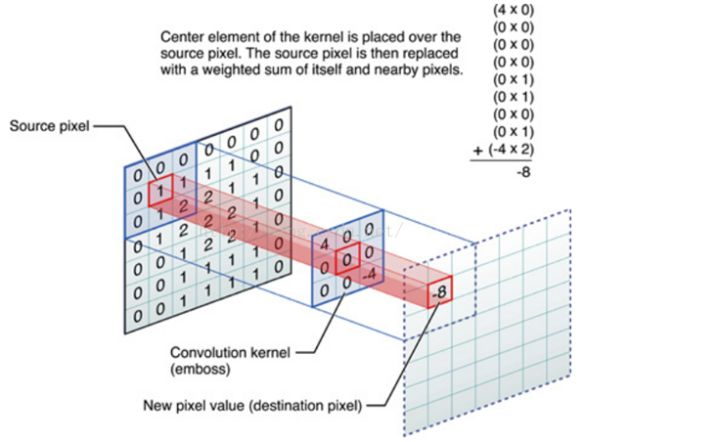
\includegraphics[height=4cm]{images/feature_map.jpg}
\end{frame}

\begin{frame}
    \frametitle{传统的CNN}
    CNN处理的图像或者视频数据中像素点(pixel)是排列成成很整齐的矩阵。\\
    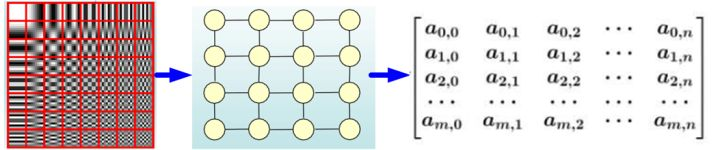
\includegraphics[height=4cm]{images/Euclidean_Structure.jpg}\\
\end{frame}

\begin{frame}
    \frametitle{为什么研究GCN}

    科学研究中还有很多Non Euclidean Structure的数据,GCN用以处理 Non Euclidean Structure 结构矩阵,如推荐系统、电子交易、计算几何、脑信号、分子结构等抽象出的图谱。这些图谱结构每个节点连接都不尽相同,有的节点有三个连接,有的节点有两个连接,是不规则的数据结构。
    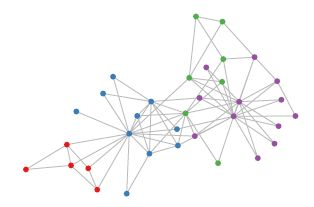
\includegraphics[height=4cm]{images/Non_Eclidean_Structure.jpg}
\end{frame}

\section{Model}
\begin{frame}
    \frametitle{GCN的推导}
    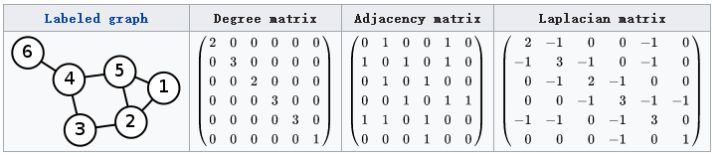
\includegraphics[height=2cm, width=10cm]{images/laplacian.jpg}\\
    对于图$G=(V, E)$,其Laplacian矩阵的定义为$L=D-A$,其中$L$是Laplacian矩阵,$D$是顶点的度矩阵(对角矩阵),对角线上元素依次为各个顶点的度,$A$是图的邻接矩阵。

\end{frame}

\begin{frame}
    \frametitle{谱分解}
    对拉普拉斯矩阵进行谱分解(特征分解)\\
    $$L= U\left(\begin{matrix}\lambda_1 & \\&\ddots \\ &&\lambda_n \end{matrix}\right) U^{-1}$$\\
    拉普拉斯矩阵是半正定对称矩阵,故其特征向量构成的矩阵为正交矩阵($UU^{T}=E$)\\
    $$L= U\left(\begin{matrix}\lambda_1 & \\&\ddots \\ &&\lambda_n \end{matrix}\right) U^{T}$$

\end{frame}

\begin{frame}
    \frametitle{傅立叶变换}
    把传统的傅里叶变换以及卷积迁移到Graph上来,主要是把拉普拉斯算子的特征函数$e^{-i\omega t}$变为Graph对应的拉普拉斯矩阵的特征向量。\\
    传统的傅立叶变换
    $$F(\omega)=\mathcal{F}[f(t)]=\int_{}^{}f(t)e^{-i\omega t} dt$$
    信号 $f(t)$ 与基函数 $e^{-i\omega t}$ 的积分。\\
\end{frame}

\begin{frame}
    \frametitle{Graph上的傅里叶变换1}
    广义的特征方程$AV=\lambda V$\\
    $A$是一种变换, $V$是特征向量或者特征函数,$\lambda$是特征值。\\
    $e^{-i\omega t}$满足:
    $$\Delta e^{-i\omega t}=\frac{\partial^{2}}{\partial t^{2}} e^{-i\omega t}=-\omega^{2} e^{-i\omega t}$$
    $e^{-i\omega t}$就是变换$\Delta$的特征函数, $\omega$和特征值密切相关。
\end{frame}

\begin{frame}
    \frametitle{Graph上的傅里叶变换2}
    考虑到拉普拉斯矩阵的特征向量\\
    $L$是拉普拉斯矩阵,$V$是其特征向量,满足下式
    $$LV=\lambda V$$
    离散积分就是一种内积形式,仿上定义Graph上的傅里叶变换:
    $$F(\lambda_l)=\hat{f}(\lambda_l)=\sum_{i=1}^{N}{f(i) u_l^*(i)}$$
    $f$是Graph上的$n$维向量,$f(i)$与Graph的顶点一一对应,$u_l(i)$表示第$l$个特征向量的第$i$ 个分量。那么特征值(频率)$\lambda_l$下的,$f$的Graph傅里叶变换就是与$\lambda_l$对应的特征向量$u_l$进行内积运算。
\end{frame}

\begin{frame}
    \frametitle{Graph上的傅里叶变换3}
    利用矩阵乘法将Graph上的傅里叶变换推广到矩阵形式:
     $$\left(\begin{matrix} \hat{f}(\lambda_1)\\ \hat{f}(\lambda_2) \\ \vdots \\\hat{f}(\lambda_N) \end{matrix}\right)=\left(\begin{matrix}\ u_1(1) &u_1(2)& \dots &u_1(N) \\u_2(1) &u_2(2)& \dots &u_2(N)\\ \vdots &\vdots &\ddots & \vdots\\ u_N(1) &u_N(2)& \dots &u_N(N) \end{matrix}\right)\left(\begin{matrix}f(1)\\ f(2) \\ \vdots \\f(N) \end{matrix}\right)$$
    即 $f$ 在Graph上傅里叶变换的矩阵形式为:$\hat{f}=U^Tf$
\end{frame}


\begin{frame}
    \frametitle{Graph上的傅里叶逆变换}
    类似地,传统的傅里叶逆变换是对频率 $\omega$ 求积分:
    $$\mathcal{F}^{-1}[F(\omega)]=\frac{1}{2\Pi}\int_{}^{}F(\omega)e^{i\omega t} d\omega$$
    迁移到Graph上变为对特征值 $\lambda_l$ 求和:
    $$f(i)=\sum_{l=1}^{N}{\hat{f}(\lambda_l) u_l(i)}$$
    推广到矩阵形式:
    $$ \left(\begin{matrix}f(1)\\ f(2) \\ \vdots \\f(N) \end{matrix}\right)= \left(\begin{matrix}\ u_1(1) &u_2(1)& \dots &u_N(1) \\u_1(2) &u_2(2)& \dots &u_N(2)\\ \vdots &\vdots &\ddots & \vdots\\ u_1(N) &u_2(N)& \dots &u_N(N) \end{matrix}\right) \left(\begin{matrix} \hat{f}(\lambda_1)\\ \hat{f}(\lambda_2) \\ \vdots \\\hat{f}(\lambda_N) \end{matrix}\right)$$
    即$f$在Graph上傅里叶逆变换的矩阵形式为:$f=U\hat{f}$
\end{frame}

\begin{frame}
    \frametitle{推广卷积1}
    函数卷积的傅里叶变换是函数傅立叶变换的乘积\\
    对于函数$f(t)$与$h(t)$两者的卷积是其函数傅立叶变换乘积的逆变换:\\
    $$f*h=\mathcal{F}^{-1}\left[ \hat{f}(\omega)\hat{h}(\omega) \right]=\frac{1}{2\Pi}\int_{}^{} \hat{f}(\omega)\hat{h}(\omega)e^{i\omega t} d\omega"$$
    类比到Graph上并把傅里叶变换的定义带入,$f$与卷积核$h$在Graph上的卷积可按下列步骤求出:\\
    $f$的傅里叶变换为$\hat{f}=U^Tf$\\
    卷积核$h$的傅里叶变换写成对角矩阵的形式即为:
    $$\left(\begin{matrix}\hat h(\lambda_1) & \\&\ddots \\ &&\hat h(\lambda_n) \end{matrix}\right)$$
    $\hat{h}(\lambda_l)=\sum_{i=1}^{N}{h(i) u_l^*(i)}$是卷积核$h$在Graph上的傅里叶变换。

\end{frame}

\begin{frame}
    \frametitle{推广卷积2}
    两者的傅立叶变换乘积即为:
    $$\left(\begin{matrix}\hat h(\lambda_1) & \\&\ddots \\ &&\hat h(\lambda_n) \end{matrix}\right)U^Tf$$
    再乘以$U$求两者傅立叶变换乘积的逆变换,则求出卷积:\\
    $$(f*h)_G= U\left(\begin{matrix}\hat h(\lambda_1) & \\&\ddots \\ &&\hat h(\lambda_n) \end{matrix}\right) U^Tf \qquad(1)$$

\end{frame}

\section{paper}

\begin{frame}
    \frametitle{T-GCN}
    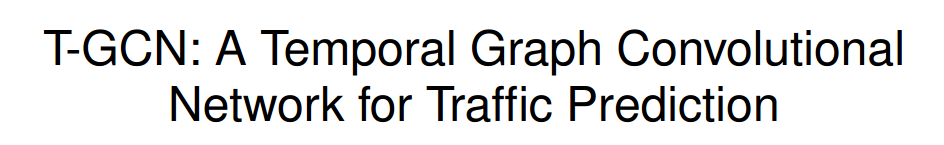
\includegraphics[height=2cm, width=10cm]{images/paper.png}\\
    To capture the spatial and temporal dependence simultaneously, we propose a novel neural network-based traffic forecasting method, the \textbf{temporal graph convolutional network (T-GCN) model}, which is in combination with the \textbf{graph convolutional network (GCN)} and \textbf{gated recurrent unit (GRU)}. Specifically, the \textbf{GCN} is used to learn complex topological structures to capture \textbf{spatial dependence} and the \textbf{GRU} is used to learn dynamic changes of traffic data to capture \textbf{temporal dependence}. Then, the T-GCN model is employed to traffic forecasting based on the urban road network.

\end{frame}

\begin{frame}
    \frametitle{Overview}
    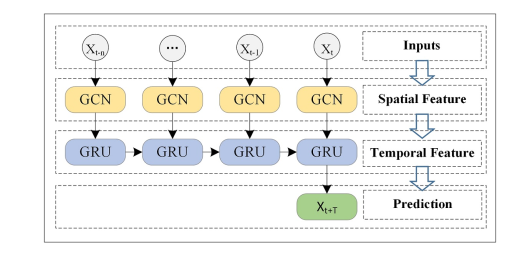
\includegraphics[height=5cm, width=8cm]{images/overview.png}\\


\end{frame}

\begin{frame}
    \frametitle{topological}
    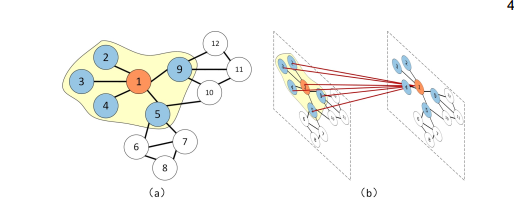
\includegraphics[height=5cm, width=10cm]{images/topological.png}\\
\end{frame}

\begin{frame}
    \frametitle{topological}
    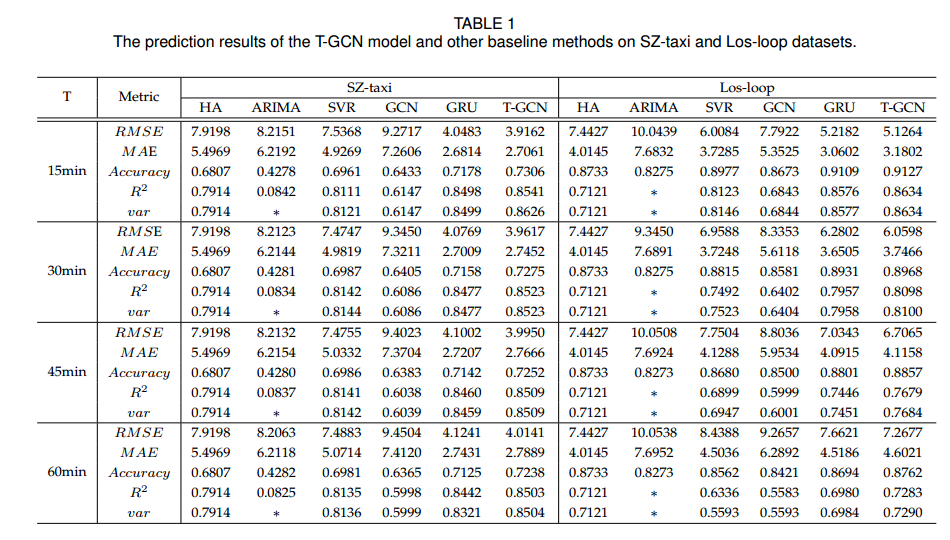
\includegraphics[height=5cm, width=10cm]{images/experiments.png}\\
\end{frame}

\section{结论}

\begin{frame}
    \frametitle{未来的展望}
    使用图卷积进行时空联合分析?\\
    结合attention?\\
\end{frame}

\end{document}